\documentclass{../exercisesheet}

\title{Datenkommunikation und Informationssysteme, Übung 6}
\author{
    Domenic Quirl \\ 354437
    \and
    Julian Schakib \\ 353889
    \and 
    Daniel Schleiz \\ 356092
}

\renewcommand{\Exercise}{Aufgabe}
\date{Übungsgruppe 14}

\usepackage{float}
%\usepackage{siunitx}
\usepackage{color}
\usepackage{multirow}
\usepackage{float}

\begin{document}
\maketitle
\pointtable


\begin{exercise}{4}
\begin{subexercise}

\end{subexercise}
\begin{subexercise}

\end{subexercise}
\begin{subexercise}

\end{subexercise}
\end{exercise}


\begin{exercise}{6}
\begin{subexercise}
Es werden Bezeichnungen wie TL für Total Length gemäß Folie IV-50 genutzt.\\
	Router 1 sendet 3 Fragmente:
	\begin{itemize}
	\item TL=1228 ID=42 MF=1 Offset=0
	\item TL=1228 ID=42 MF=1 Offset=151
	\item TL=404 ID=42 MF=0 Offset=302
	\end{itemize}
	Von Router 2 zum Empfänger müssen die ersten beiden Fragmente nochmal fragmentiert werden, da diese die MTU überschreiten. Insgesamt sendet Router 2 also folgende
	5 Fragmente:
	\begin{itemize}
	\item TL=660 ID=42 MF=1 Offset=0
	\item TL=588 ID=42 MF=1 Offset=80
	\item TL=660 ID=42 MF=1 Offset=151
	\item TL=588 ID=42 MF=1 Offset=231
	\item TL=404 ID=42 MF=0 Offset=302
	\end{itemize}
\end{subexercise}
\begin{subexercise}
Unter der Annahme, dass die ID's bei 0 beginnen, existieren also $2^{16}$ verschiedene ID's. Falls innerhalb von einer Sekunde mehr als $2^{16}$ Pakete verschickt werden, ist das erste
noch nicht angekommen und es wird eine ID doppelt verteilt. Die Datenrate darf somit nur maximal $\frac{2^{16} \cdot 1500 \text{ Byte}}{1\text{s}}= 
98304000 \text{ Byte/s}= 98,305 \text{ MByte/s}$ betragen.
\end{subexercise}
\begin{subexercise}
Dies ist nicht problematisch, da in den IP-Headern der Fragmente neben der ID noch ebenfalls die Destination Address steht, wodurch die Empfänger trotzdem eindeutig die Fragmente
wieder zusammenbauen können.
% Ich evrstehe irgendwie die Frage nichr: Soll ein Paket, welches für z.B. Empfänger 1 bestimmt war, bei Empfänger 2 ankommen, mit gleicher ID wie das eigentlich für 2 bestimmte Paket?
\end{subexercise}
\begin{subexercise}
Ein Vorteil besteht darin, dass Zwischenstationen bei einer Übertragung entlastet werden, da die MTU für einen Pfad nur einmal berechnet werden muss und danach gecached wird, 
wodurch die Zwischenstationen im Allgemeinen weniger fragmentieren müssen. Damit lassen sich eventuell höhere Datenraten erzielen.\\
Ein Nachteil sind eventuell verloren gehende Pakete aufgrund von z.B. Firewalls: Falls beim Lernprozess der Path MTU Discovery an einer Stelle die MTU überschritten wird, aber
die darauf folgende ICMP-Meldung an den Sender durch eine Firewall abgefangen wird, denkt der Sender, das Paket sei angekommen, obwohl es verworfen wurde.
\end{subexercise}
\end{exercise}


\begin{exercise}{5}
\begin{subexercise}
\begin{figure}[H]
  \centering
  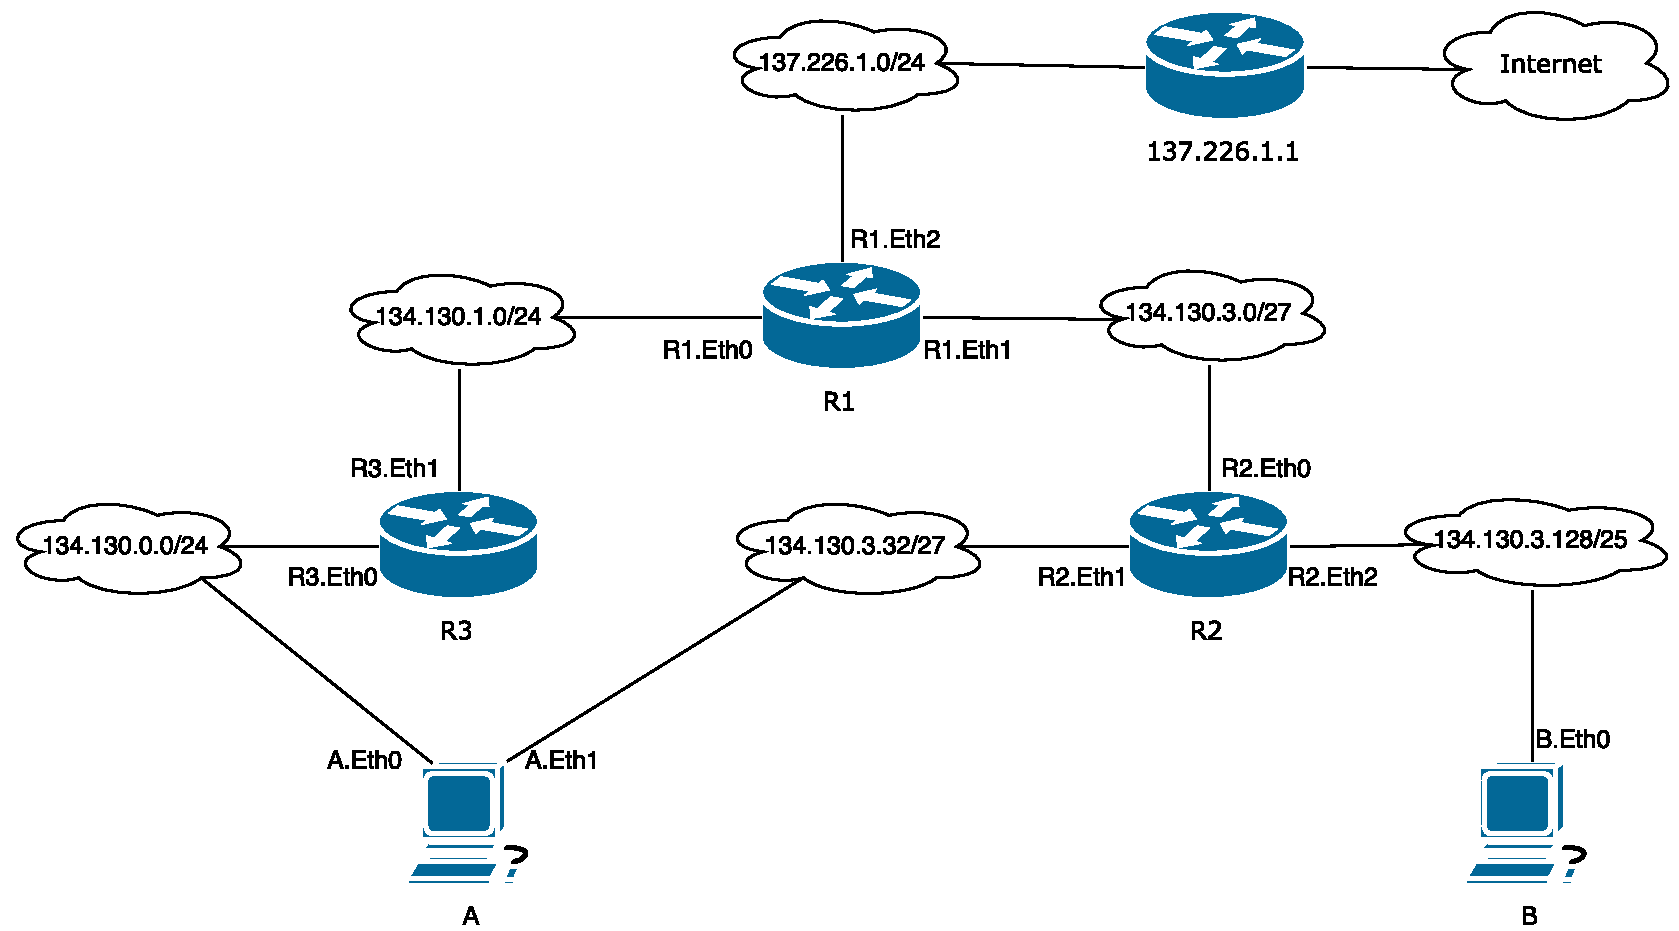
\includegraphics[width=\textwidth]{a3_network.pdf}
\end{figure}
\end{subexercise}
\begin{subexercise}
%Der längste Match der IP-Adresse von B in der Tabelle von A besteht bei \texttt{0.0.0.0/0}, somit sendet A durch ETH0.\\ \ \\
%\texttt{Request A.ETH0 134.130.0.152} - 
%\texttt{} - 
\end{subexercise}
\end{exercise}


\end{document}

